%\pagebreak
\chapter{Hubschrauber für Infanteristen}
\label{HuFIn}
\subsection{Hubschrauber im Einsatz}
	Pro: 
	\vspace{-2mm}
	\begin{itemize}
		\item Observation im Bereich
		\item Aufnehmen und Absetzen von Trupps
		\item Tarnung
		\item Rapid Reaction
		\item \ac{CAS}
	\end{itemize}

	Contra: 
	\vspace{-2mm}
	\begin{itemize} 
		\item Größere Verwundbarkeit (größeres Waffenkontingent)
		\item Laut
	\end{itemize}

\subsection{Aufgaben der Infanterie im Hubschrauber}
	Aufgabe der Infanterie im Flug ist es nach allen Bedrohungen Ausschau zu halten. Sei es Gewehrfeuer, Raketen, Positionen feindl. Kräfte, Hindernissen oder jeglicher anderer Gefahr für das Fahrzeug. Der Pilot ist immer zu informieren und auf dem Laufenden zu halten! Überflüssige Gespräche sollten vermieden werden.

\subsection{Koordination}
	Bevor es in den Einsatz geht sind Vorkehrungen zu treffen. 
		\begin{itemize} 
			\item Welcher Trupp kommt in welchen Hubschrauber? 
			\item Welcher Hubschrauber geht zu welcher \ac{LZ}? 	
			\item Die Kräfte sind möglichst gleich und redundant zu verteilen wenn möglich.
		\end{itemize}

	Bei Abholung bestimmt der Truppführer, wenn benötigt bzw. möglich, einen Einweiser und das letzte Sicherungsglied.

\subsection{Bereitstellen einer \acf{LZ}}
	Eine ideale \ac{LZ} bietet genug Deckung, sowohl für den Trupp als auch für den Hubschrauber. Ein minimale Landefläche beträgt $25m * 25m$ (ohne viele Hindernisse) und in dieser eine absolut freie Fläche von minimal $5 * 5$ Meter. Dies kann je nach Hubschrauber variieren. Je flacher das Gelände ist, desto weiter muss der Hubschrauber von feindlichen Kräften entfernt landen um die Sicherheit zu garantieren. Ein hügeliges Gelände erlaubt nähere Landemanöver, wenn das Terrain eine Deckung des Hubschraubers erlaubt.
	\begin{figure}[htbp]
		\centering
		\includegraphics[width=0.95\linewidth]{../img/advanced/hubschrauber_+_infanterie/landezone}
	\end{figure}	

	Für den Anflugbereich wird angestrebt, einen möglichst sicheren (am besten Unsichtbaren) Anflugbereich zu ermöglichen. Trupps werden wenn möglich >>direkt in der Deckung<< abgeladen oder aufgenommen. Es ist erstrebenswert das der Hubschrauber während des Landemanövers über möglichst viel Deckung verfügt. Je näher am Gegner gelandet werden muss, desto größer ist die Gefahr.
	\begin{figure}[htbp]
		\centering
		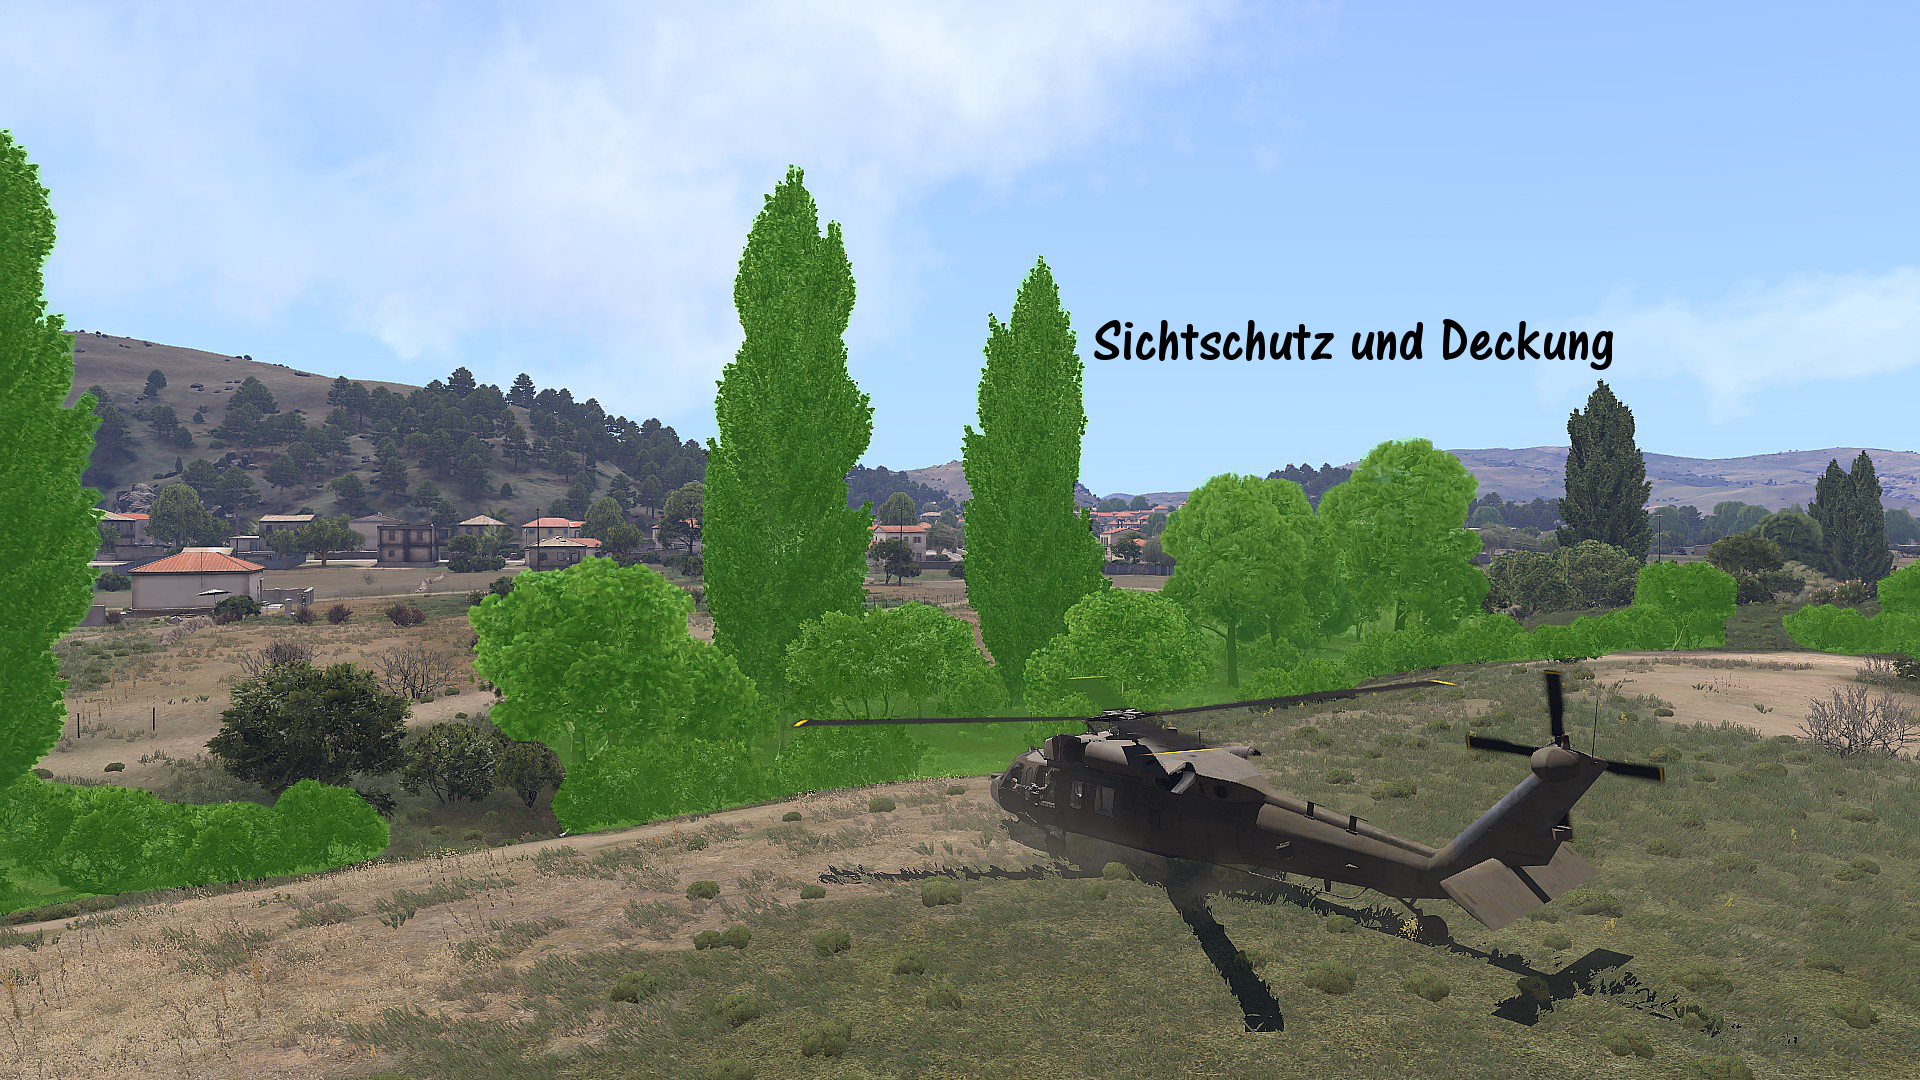
\includegraphics[width=0.95\linewidth]{../img/advanced/hubschrauber_+_infanterie/verdeckte-landung}
	\end{figure}	
	\begin{figure}[htbp]
		\centering
		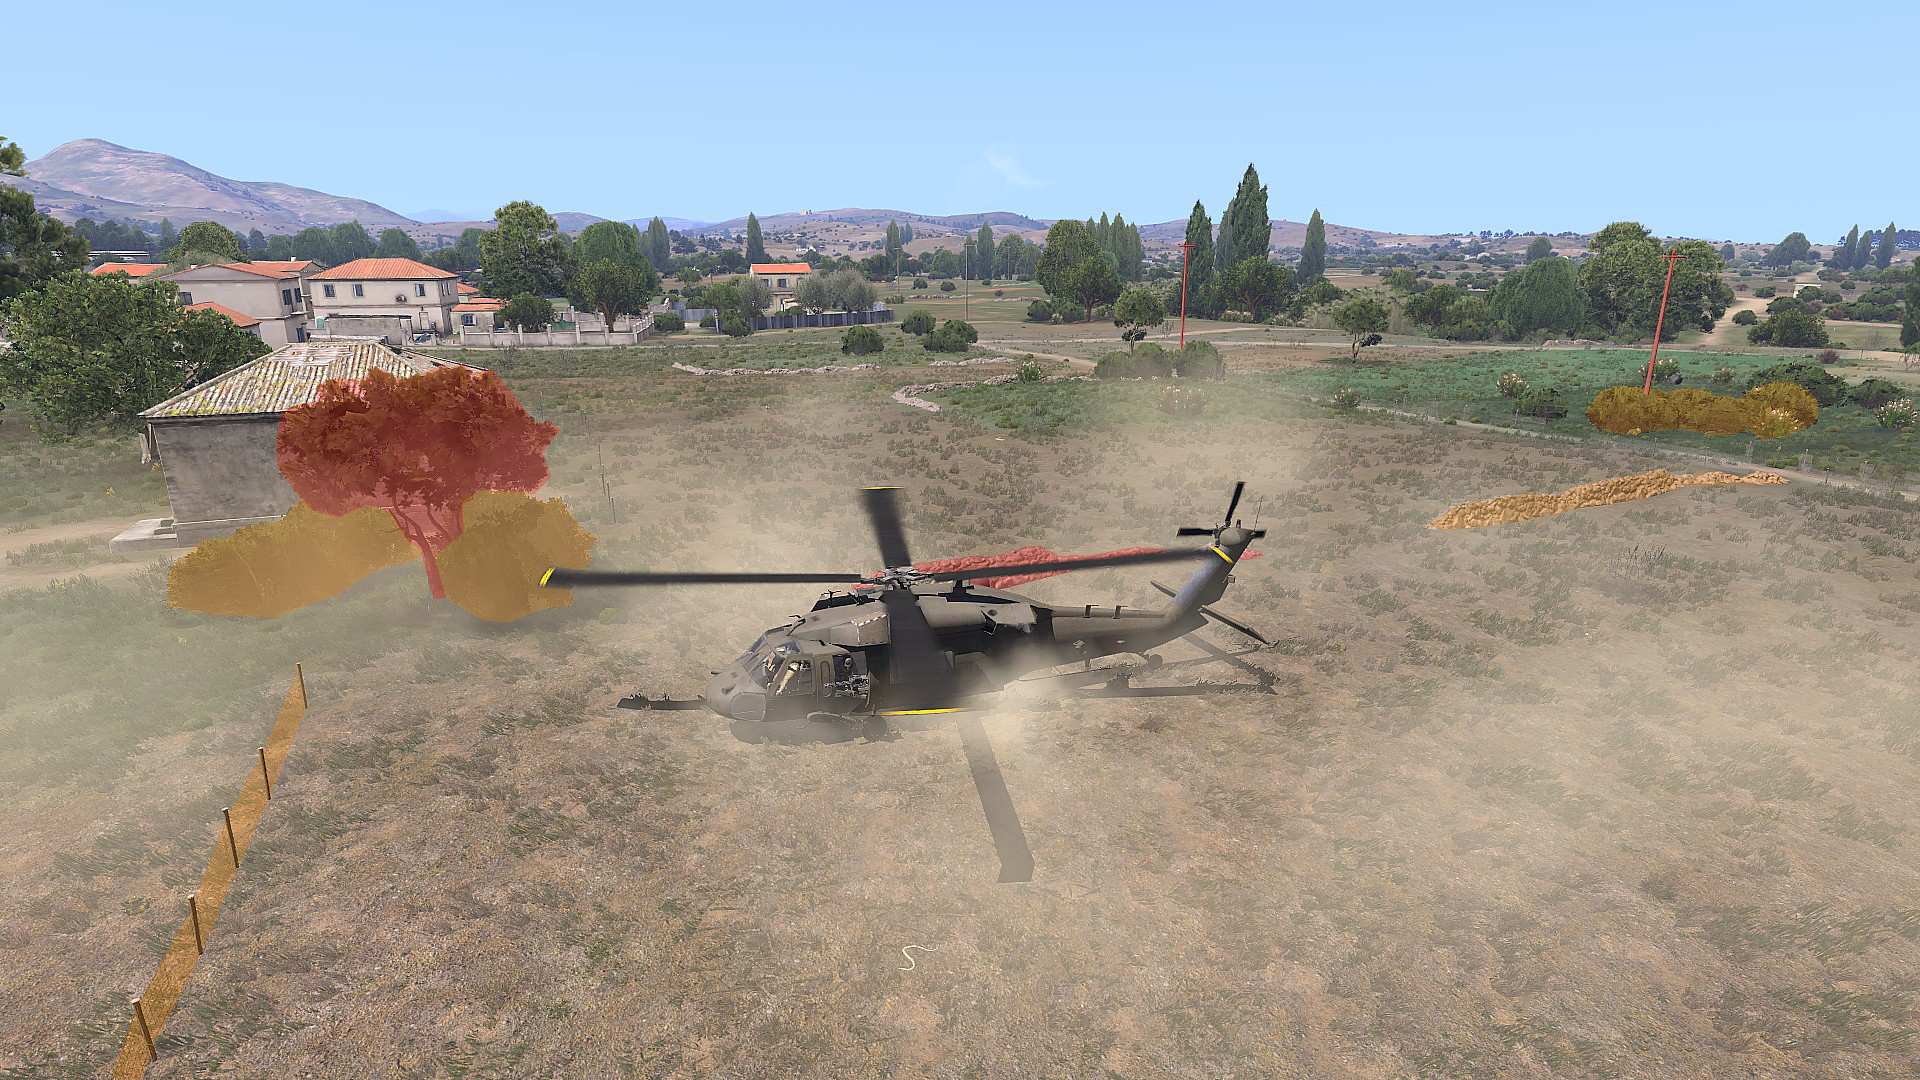
\includegraphics[width=0.95\linewidth]{../img/advanced/hubschrauber_+_infanterie/bodenlesen-sicht-pilot}
	\end{figure}
	\begin{figure}[htbp]
		\centering
		\includegraphics[width=0.95\linewidth]{../img/advanced/hubschrauber_+_infanterie/bodenlesen-sicht-pilot-2}
	\end{figure}
	
	Weiterhin sollten alle möglichen Gefahren im Bereich der Landezone analysiert werden. Gibt es feindl. Patrouillen im Gebiet? Sind Anti-Air Waffen des Feindes im Gebiet gemeldet worden?
	\begin{figure}[htbp]
		\centering
		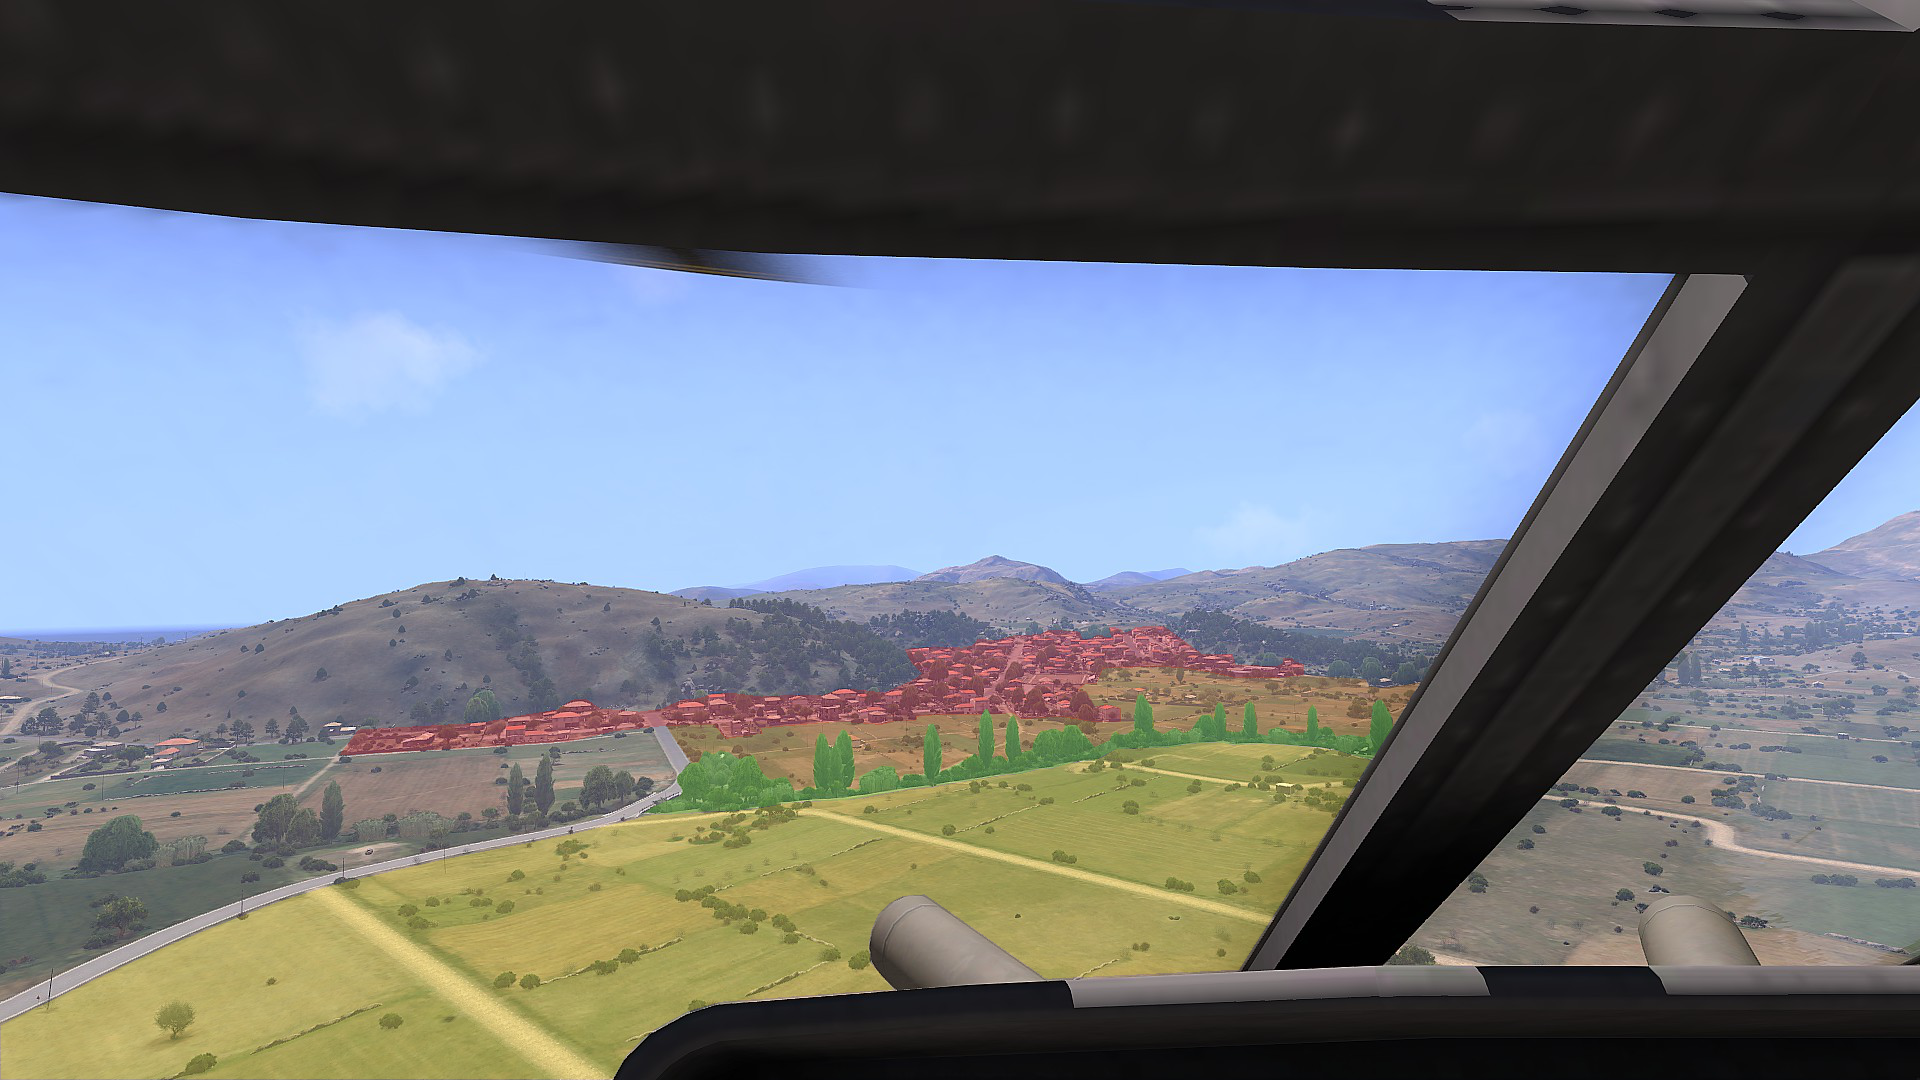
\includegraphics[width=0.95\linewidth]{../img/advanced/hubschrauber_+_infanterie/sicht-pilot}
	\end{figure}
			
	Zum Abschluss wird eine Ersatz \ac{LZ} geplant und vermerkt. Sollte irgendetwas unvorhergesehenes passieren kann problemlos auf diese ausgewichen werden.

\subsection{Extraktion per Hubschrauber}
 	\begin{itemize} 
		\item Wenn die Landezone ausgesucht und definiert wurde, wird der Hubschrauber angefordert. Der Hubschrauber nimmt Kontakt per Funk auf, wenn er in das Gebiet des Trupps kommt und fordert die benötigten Maßnahmen an.

		\item Sobald der Hubschrauber in Reichweite ist, ist er auch in der Verantwortung des Infanterietrupps, welcher ihn angefordert hat. Die Infanterie muss den Hubschrauber um jeden Preis schützen!

		\item Sobald die Funk-Kommunikation hergestellt wurde muss der Hubschrauber mit Informationen vom Squadleader versorgt werden. Stichwort: Situationsbericht. Ist die Landezone Heiß/Kalt? Gibt es Bedrohungen im Gebiet die vorher nicht bekannt waren?

		\item Eine Basislandmarke, welche bei der Orientierung zur Suche der Landezone helfen kann, ist empfehlenswert. (Beispiel: Nördlich vom Sportplatz/Kirche)

		\item Wenn der Heli an einem etwas weiteren Ort entfernt sicherer landen kann und die Infanterie dafür etwas laufen muss ist das ein durchaus akzeptables Risiko.

		\item Wird eine spezielle Landezone gewählt oder muss unkonventionell gelandet werden sind die Gründe des Manövers dem Piloten mitzuteilen. (Wir landen am Südhang, da von Norden mit Feindfeuer zu rechnen ist.)

		\item Wenn der Hubschrauber Rauch verlangt wird dieser geworfen und wenn verfügbar/benötigt macht sich der Einweiser bereit.

		\item Der Hubschrauber meldet den Touchdown über Funk.

		\item Ghosthawk: Im finalen Anflug geben die Türschützen Unterdrückungsfeuer auf jegliche Bedrohungen. Es wird so lange geschossen, bis der Hubschrauber den Boden berührt. Dann nur noch im Notfall. Sobald der Hubschrauber wieder abgehoben hat, wird das Unterdrückungsfeuer wieder aufgenommen.

		\item Die Annäherung an den Hubschrauber erfolgt frontal, mit einem finalen Schwenk zum seitlichen Einstieg. Dies bietet mehr Sicherheit und Schutz, ebenfalls wird dadurch Kreuzfeuer der Türschützen vermieden.

		\item >>Loadmaster<< gibt Pilot Freigabe. (oder Squadleader, je nach Truppstruktur / Verladestruktur)
	\end{itemize}

\subsection{Eingeflogen werden}
	\begin{itemize} 
		\item Der Pilot wurde über die \ac{LZ} informiert. Die Verantwortungsbereiche sind verteilt. Dann wird ein Sammelpunkt nahe der \ac{LZ} für den Abgesetzten Trupp definiert. Sobald der Infanterietrupp abgeladen wurde, wird sich unverzüglich zum Sammelpunkt begeben.

		\item Höchste Aufmerksamkeit beim finalen Anflug.

		\item Helikopter mit Seitenbewaffnung: Die Türschützen übernehmen das Unter\-drückungs\-feuer bis der Hubschrauber den Boden berührt.

		\item Der Pilot bespricht mit dem Loadmaster den Touchdown.

		\item Die Infanterie gibt ihr grünes Licht, das alle abgesessen haben und der Hubschrauber startet durch.

		\item Zeitfaustregel: Unter 1 Min. für ein Platoon!
	\end{itemize}

\subsection{Das Worst Case-Szenario}
	\begin{itemize}
		\item \ac{LZ} Abbruch obliegt dem Piloten!
		\item Pilot hat das aller letzte Wort!
		\item Unter plötzlichem Beschuss die Deckung des Hubschraubers wenn nötig mit Rauch unterstützen.
		\item Wenn der Pilot einen Notfall deklariert, werden alle Pläne/Aktionen verworfen und das Sichern des Überlebens wird Priorität Nummer 1!
	\end{itemize}

\subsection{Finale Informationen zum Anweiser}
	Der Einweiser ist der Draht zum Hubschrauber.

	Wenn der Einweiser im Einsatz ist, ist dieser für den Hubschrauber verantwortlich. Dies bedeutet ebenfalls bei schwierigem Gelände dieses zu überwachen und bei Gefahr einen >>Abbruch!<< Befehl zu geben. In diesem Fall wird das Landemanöver abgebrochen und mit Rücksprache ein Neues einzuleiten.

\subsection{Beispielablaufplan: Anrufen eines Transportes}
	\begin{itemize}
		\item \ac{KT} funkt mit OPL Transportanfrage aus
    		\item \ac{OPL} gibt Transportfreigabe - erteilt Ausführungsbefehl
    		\item KT >>Anweiser<< nimmt gemeinsam mit Hubschrauber auf Hubschrauber \ac{SR} Kontakt auf
    		\item Absprache Auftrag Trupp mit Hubschrauber - Landmarke/Anflug
			\item Hubschrauber meldet Anflug
    		\item Hubschrauber fordert ggf. Rauchmarkierung
    		\item Hubschrauber fordert Anweisung
    		\item Touchdown
    		\item Aufsitzen
    		\item >>Kampftrupp komplett.<< / >>Los! Los! Los!<< vom Truppführer
    		\item Abflug (Anweiser Verantwortung endet)
	\end{itemize}
